% The Hesse configuration = the affine plane over F_3: 9 points, 12 lines of 3 points; straight lines are drawn straight, the 4 'broken' lines as circles.
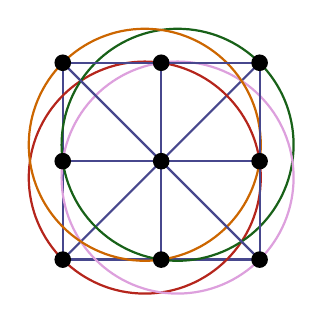
\begin{tikzpicture}[scale=1.25]
\draw[MidnightBlue!80,thick] (0.0000,0.0000) -- (0.0000,2.0000);
\draw[MidnightBlue!80,thick] (0.0000,0.0000) -- (2.0000,0.0000);
\draw[MidnightBlue!80,thick] (0.0000,0.0000) -- (2.0000,2.0000);
\draw[BrickRed,thick] (0.8333,0.8333) circle (1.1785);
\draw[ForestGreen!70!black,thick] (1.1667,1.1667) circle (1.1785);
\draw[MidnightBlue!80,thick] (0.0000,1.0000) -- (2.0000,1.0000);
\draw[Plum,thick] (1.1667,0.8333) circle (1.1785);
\draw[orange!80!black,thick] (0.8333,1.1667) circle (1.1785);
\draw[MidnightBlue!80,thick] (0.0000,2.0000) -- (2.0000,0.0000);
\draw[MidnightBlue!80,thick] (0.0000,2.0000) -- (2.0000,2.0000);
\draw[MidnightBlue!80,thick] (1.0000,0.0000) -- (1.0000,2.0000);
\draw[MidnightBlue!80,thick] (2.0000,0.0000) -- (2.0000,2.0000);
\fill (0.0000,0.0000) circle (2.4pt);
\fill (0.0000,1.0000) circle (2.4pt);
\fill (0.0000,2.0000) circle (2.4pt);
\fill (1.0000,0.0000) circle (2.4pt);
\fill (1.0000,1.0000) circle (2.4pt);
\fill (1.0000,2.0000) circle (2.4pt);
\fill (2.0000,0.0000) circle (2.4pt);
\fill (2.0000,1.0000) circle (2.4pt);
\fill (2.0000,2.0000) circle (2.4pt);
\end{tikzpicture}
